%\section{شبیه‌سازی کانال رول استند در حضور کنترل‌کننده \lr{LQDG}}\label{roll_LQDG_section_simulation}
در این بخش به بررسی عملکرد چهارپره در حضور کنترل‌کننده \lr{LQDG} پرداخته می‌شود. کنترل‌کننده \lr{LQDG} در بخش
\ref{LQDG}
بررسی شده‌است.
 در شبیه‌سازی برای بهینه‌سازی ضرایب وزنی مانند قسمت قبل عمل شده‌است.
%  \lr{LQDG} از روش بهینه‌سازی
%\lr{TCACS}
%استفاده شده‌است.
%تابع هزینه \lr{TCACS} به‌صورت
%\lr{ITSE}
%در نظر گرفته شده‌است. ضرایب وزنی خروجی بهینه‌سازی در پایین آورده شده‌است.
\begin{equation}
	\boldsymbol{Q_{LQDG}} = \begin{bmatrix}
		100 & 0\\
		0 & 0.078
	\end{bmatrix}, \quad R_{1_{LQDG}} =  1, \quad R_{2_{LQDG}} =  99.96
\end{equation}
در گام بعد، با حل معادله
(\ref{coupled_riccatti_LQDG})
(برای سادگی ماتریس‌های وزنی $\boldsymbol{\dot{Q}_{2}}$ و $\boldsymbol{\dot{Q}_{1}}$مساوی در نظر گرفته شده‌است)
ماتریس
$\boldsymbol{{K}_1}$
به‌صورت زیر به دست می‌آید.
\begin{equation}
	\boldsymbol{K_1} = \begin{bmatrix}
		
		286.0470  & 39.1188\\
		39.1188   & 8.8510\\
	\end{bmatrix}
\end{equation}
در نهایت فرمان کنترلی بهینه بازیکن اول از رابطه
(\ref{LQDG_u})
به‌صورت زیر به دست می‌آید.
\begin{equation}
	u_1 = -\begin{bmatrix}
		39.1188   & 8.8510
	\end{bmatrix}\boldsymbol{x}(t)
\end{equation}

\begin{figure}[H]
	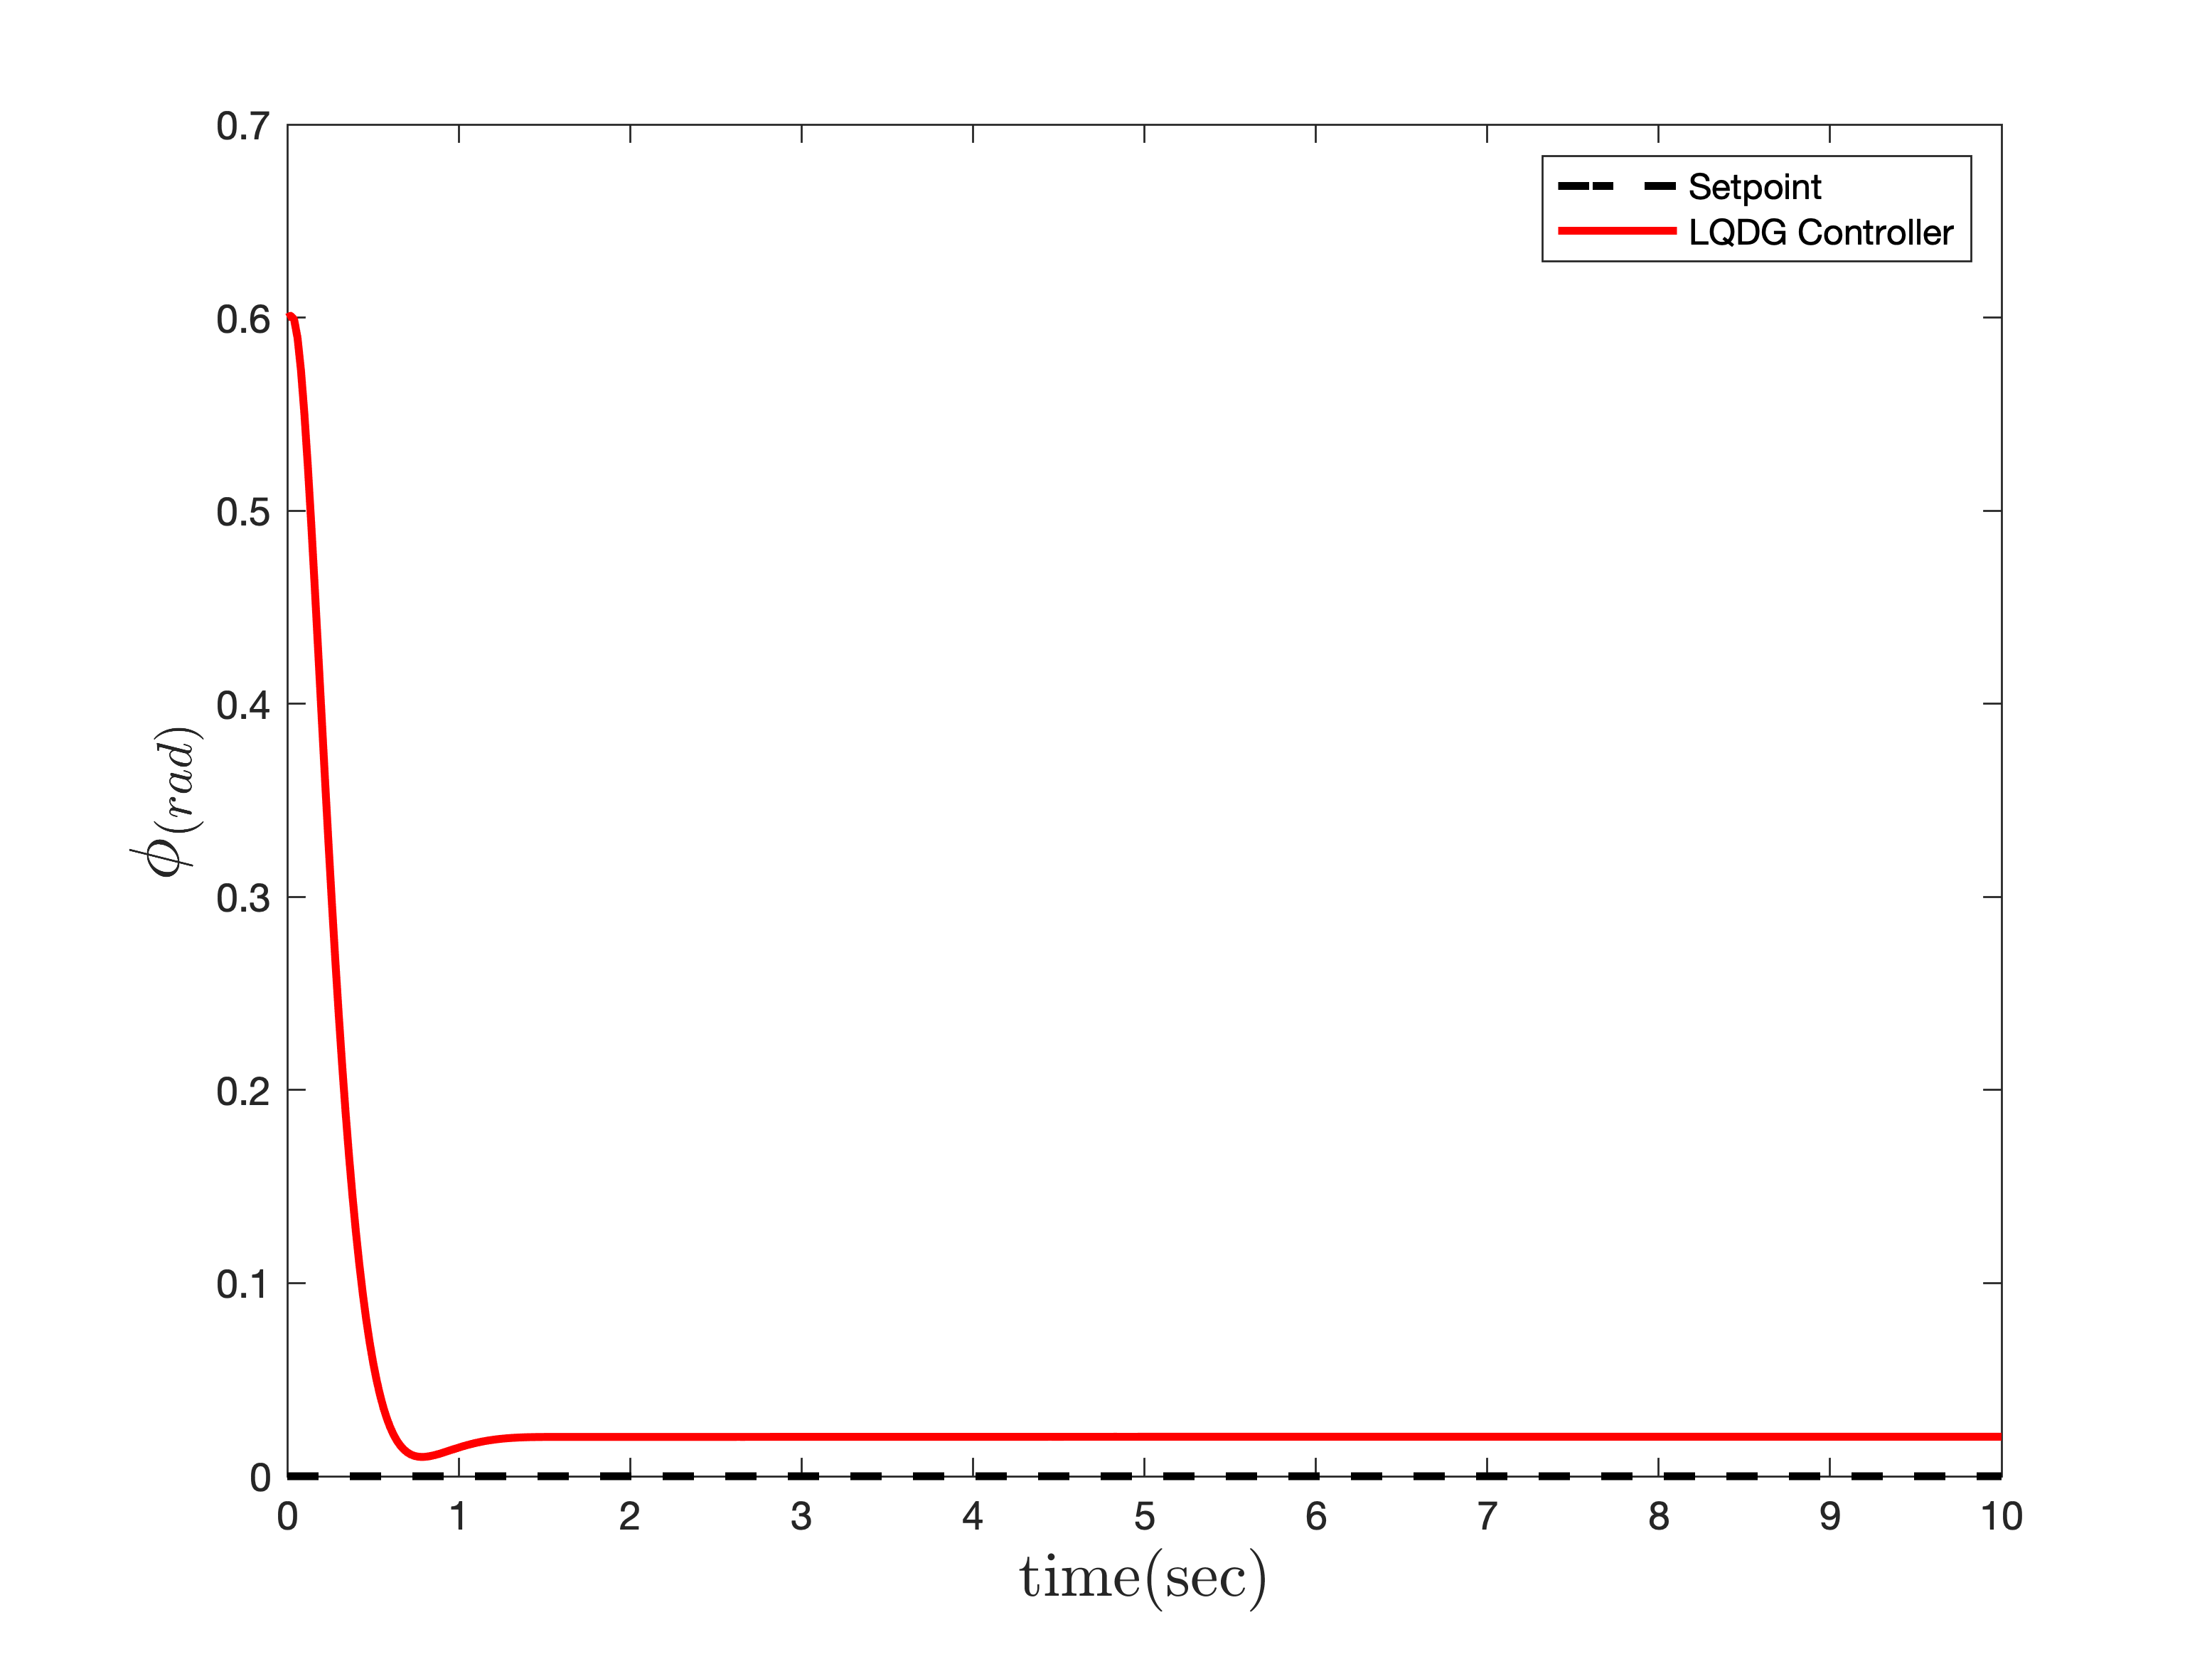
\includegraphics[width=.48\linewidth]{../Figures/MIL/LQDG/Roll/lqdg_roll_nn.png}
	\centering
	\caption{عملكرد کنترل‌کننده \lr{LQDG} در کنترل زاويه رول (تعقیب ورودی صفر)}
	\label{lqdg_roll_fig_simulation}
\end{figure}
\begin{figure}[H]
	\centering
	\subfigure[موتور شماره دو]{
		\centering
		\includegraphics[width=.45\linewidth]{../Figures/MIL/LQDG/Roll/lqdg_roll_Omega_2_nn.png}
	}
	\subfigure[موتور شماره چهار]{
		\centering
		\includegraphics[width=.45\linewidth]{../Figures/MIL/LQDG/Roll/lqdg_roll_Omega_4_nn.png}
	}
	\caption{‫‪فرمان کنترلی موتورها در کنترل زاویه رول (تعقیب ورودی صفر)}
\end{figure}

همانطور که از شکل
\ref{lqdg_roll_fig_simulation}
مشخص است، زمان نشست در حدود دو ثانیه است. خطای ماندگار دارد.